\documentclass[a4paper, 11pt]{article}
\usepackage[margin=2.5cm]{geometry}

\usepackage{enumitem}
\usepackage{calc}
\usepackage{amsmath}

\usepackage{amssymb}
\usepackage{courier}
\usepackage{eurosym}
\usepackage{tikz}
\usepackage{mathtools}
\usepackage{listings}
\usepackage{color} %red, green, blue, yellow, cyan, magenta, black, white
\usepackage{algpseudocode}
\usepackage{algorithm}
\definecolor{mygreen}{RGB}{28,172,0} % color values Red, Green, Blue
\definecolor{mylilas}{RGB}{170,55,241}


\DeclareMathOperator*{\argmin}{\textbf{argmin}}
\DeclareMathOperator*{\sign}{\textbf{sgn}}
\DeclareMathOperator{\dom}{\textbf{dom}}
\DeclareMathOperator{\sgn}{\textbf{sgn}}
\newcommand{\epi}{\operatorname{epi}}

\lstset{language=Matlab,%
	%basicstyle=\color{red},
	breaklines=true,%
	morekeywords={matlab2tikz},
	keywordstyle=\color{blue},%
	morekeywords=[2]{1}, keywordstyle=[2]{\color{black}},
	identifierstyle=\color{black},%
	stringstyle=\color{mylilas},
	commentstyle=\color{mygreen},%
	showstringspaces=false,%without this there will be a symbol in the places where there is a space
	numbers=left,%
	numberstyle={\tiny \color{black}},% size of the numbers
	numbersep=9pt, % this defines how far the numbers are from the text
	emph=[1]{for,end,break},emphstyle=[1]\color{red}, %some words to emphasise
	%emph=[2]{word1,word2}, emphstyle=[2]{style},    
}
\title{Design Decisions}
\begin{document}
	\maketitle
	\subsection*{Architecture}
	Once we were given the assignment we spent considerable time hashing out a plan for our system's architecture. Given the mention of extensibility in the assignment brief we opted for a design that would involve a significant degree of decoupling between the User Interface and the implementation of the game's logic. This would allow the development of either aspect of the game without any implementation details of either main part being known by the other, tied together via the core game mechanics and a messaging system.
	\subsection*{High Level Concept}
	On a high level the architecture is as follows. Due to the turn based nature of this game and the relatively linear flow of a turn with a limited set of very basic interactions with the user we decided to implement the logic as a state machine. This state machine uses the messages sent by the UI as its stimuli and mutates the logic classes based on the current state and received information.\par 
	\noindent The UI then runs in a pair of threads. The first of these is responsible for the rendering/drawing of the current UI `screen' and runs to a set frame rate. The second thread is the action listener that reacts to button presses. This thread is responsible for changing the state of the UI based on the response messages it receives from the game logic.\par 
	\noindent The messaging interface is the decoupling intermediary between the two. It defines the communication system and handles the passing of messages without requiring any knowledge of implementation.
	
	\subsection*{GameEngine.java}
	This class is responsible for the management of the three main components in this design (UI, Logic, MessagingInterface). 
	\begin{figure}[!h]
		\centering
		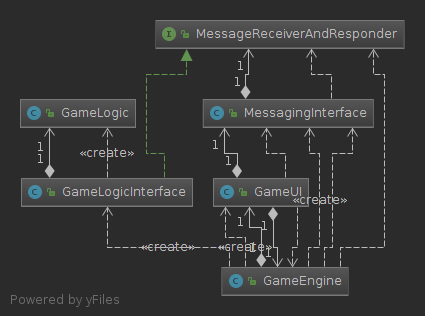
\includegraphics[scale=.45]{uml/messaging_system_uml}
		\caption{High Level UML.}
		\label{fig:high_level_uml}
	\end{figure}
	When the game begins the Interface is instantiated first, followed by the other two components which have a reference to the messaging system passed to it.
		
	\subsection*{Messaging Interface}
	The messaging interface itself is quite simple, just consisting of just one function apart from the constructor, \texttt{sendMessageAcceptResponse}. This is called by the user interface with an initial message and blocks execution until it returns with a response from the UI. When the interface is initialised it has the logic object passed to it and calls the corresponding receive message function implemented by the logic. This fulfils our objective of having each component unaware of the other's implementation. %TODO andrew you should probably write this
	
	\subsubsection*{Messages}
	Twelve messages have been implemented mostly in pairs, which represent a message from the logic and the corresponding response from the user. Where possible these messages are created using the same class and varying an enumerable message type, however some messages are of a variation on the format and require separate classes to represent them. The types of messages are denoted below along with their relationship structure.
	\begin{table}[!ht]
		\begin{flushleft} 
			\begin{tabular}{l} 
				StartupMessage\\
				SpinRequest\\
				SpinResponse\\
				LargeDecisionRequest\\
				LargeDecisionResponse\\
				OptionDecisionRequest\\
				OptionDecisionResponse\\
				AckRequest\\
				AckResponse\\
				EndGameMessage\\
				UIConfigMessage\\
				SpinResult\\	
			\end{tabular}
		\end{flushleft}
	\end{table}
	\begin{figure}[!h]
		\centering
		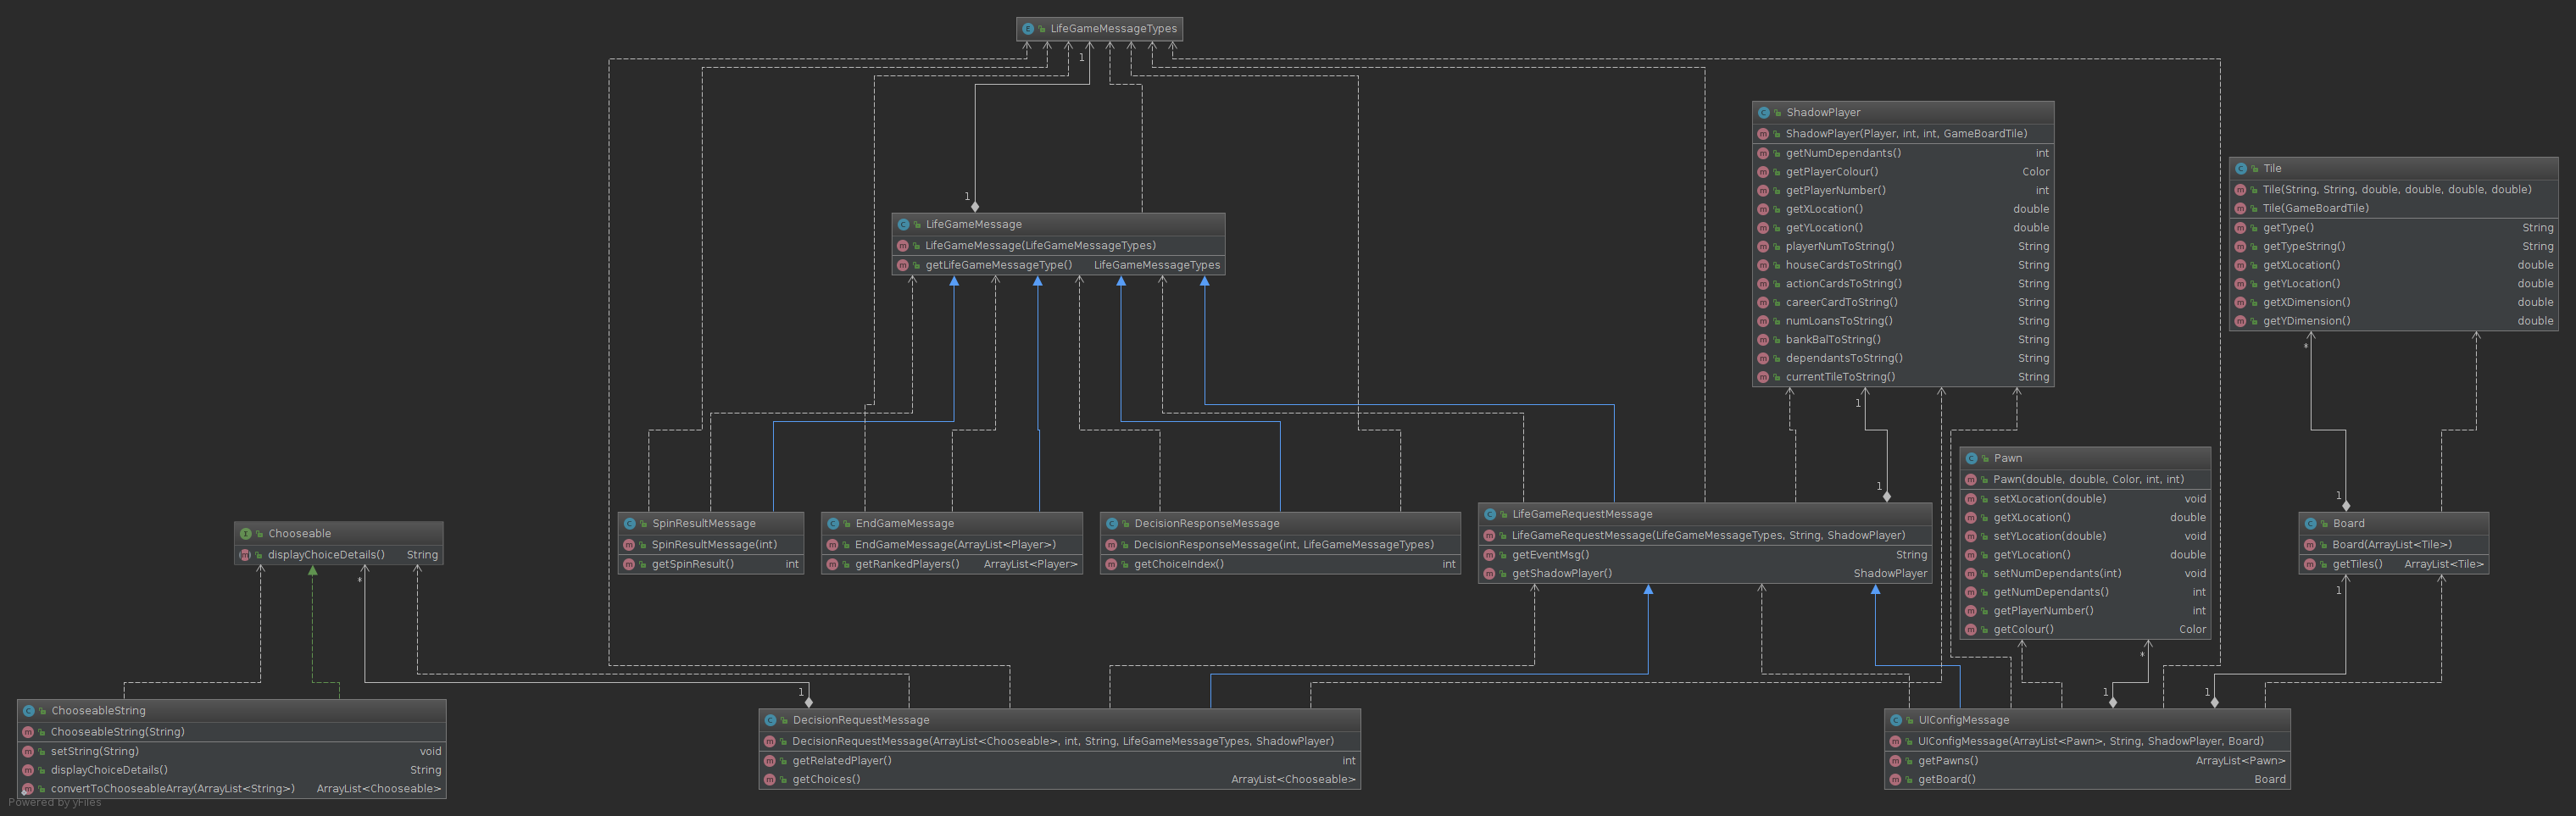
\includegraphics[scale=.125]{uml/messaging_internals_uml}
		\caption{Messaging System Internals.}
		\label{fig:messages_uml}
	\end{figure}
	\subsubsection*{ShadowPlayer}
	\texttt{ShadowPlayer} is how the messaging system represents the attributes relating to the player object that are of interest to the person controlling that pawn, such as bank balance or the current career card.
	In order to abide by the decoupling principle the player object is not directly accessed or sent to the interface, however a representation of this data is sent instead that hides the implementation details.
	As far as the UI is concerned this \texttt{ShadowPlayer} outputs a series of strings corresponding to each piece of information.
	The logic is able to construct a \texttt{ShadowPlayer} based on the player objects and send them as an attachment to messages when required.
	\subsubsection*{Tile/Pawn}
	\texttt{Tile} and \texttt{Pawn} are the simplest part of this interface, used only when the game is being set up in order to send the coordinates, sizes, types of the tiles and the colours of the respective players to the interface so that they can be drawn.
	
	\subsection*{State Machine}
	As previously mentioned due to the turn based nature of this game and the relatively linear flow of a turn with a limited set of very basic interactions with the user we decided to implement the logic as a state machine. This state machine uses the messages sent by the UI as its stimuli and mutates the logic classes based on the current state and received information. The original state transition diagram can bee seen in Figure \ref{fig:state_machine}.\\
	The idea we had in mind essentially as a pair of state machines with one inside the other. The outside one would handle the overall game state, with actions such as handling the turns, spinning, movement etc. The inner state machine then would be called into action only when we needed to handle more complex turn logic, such as the spin-to-win tile or the acquisition of houses.\\
	The way in which we managed this was as follows:\\
	When the player had spun the wheel at the start of their turn the logic then enters \textit{Handle Player Move State}. Once in this state the logic establishes, depending on the tile landed on, what the next state must be. If the state is not complex we handle the turn interaction in \textit{Handle Player Move State} itself. However if the state is more complicated the state machine then transitions into a state corresponding to that tile's action, which takes over the handling of user input until the tile action sequence has been completed.
	\begin{figure}[!h]
		\centering
		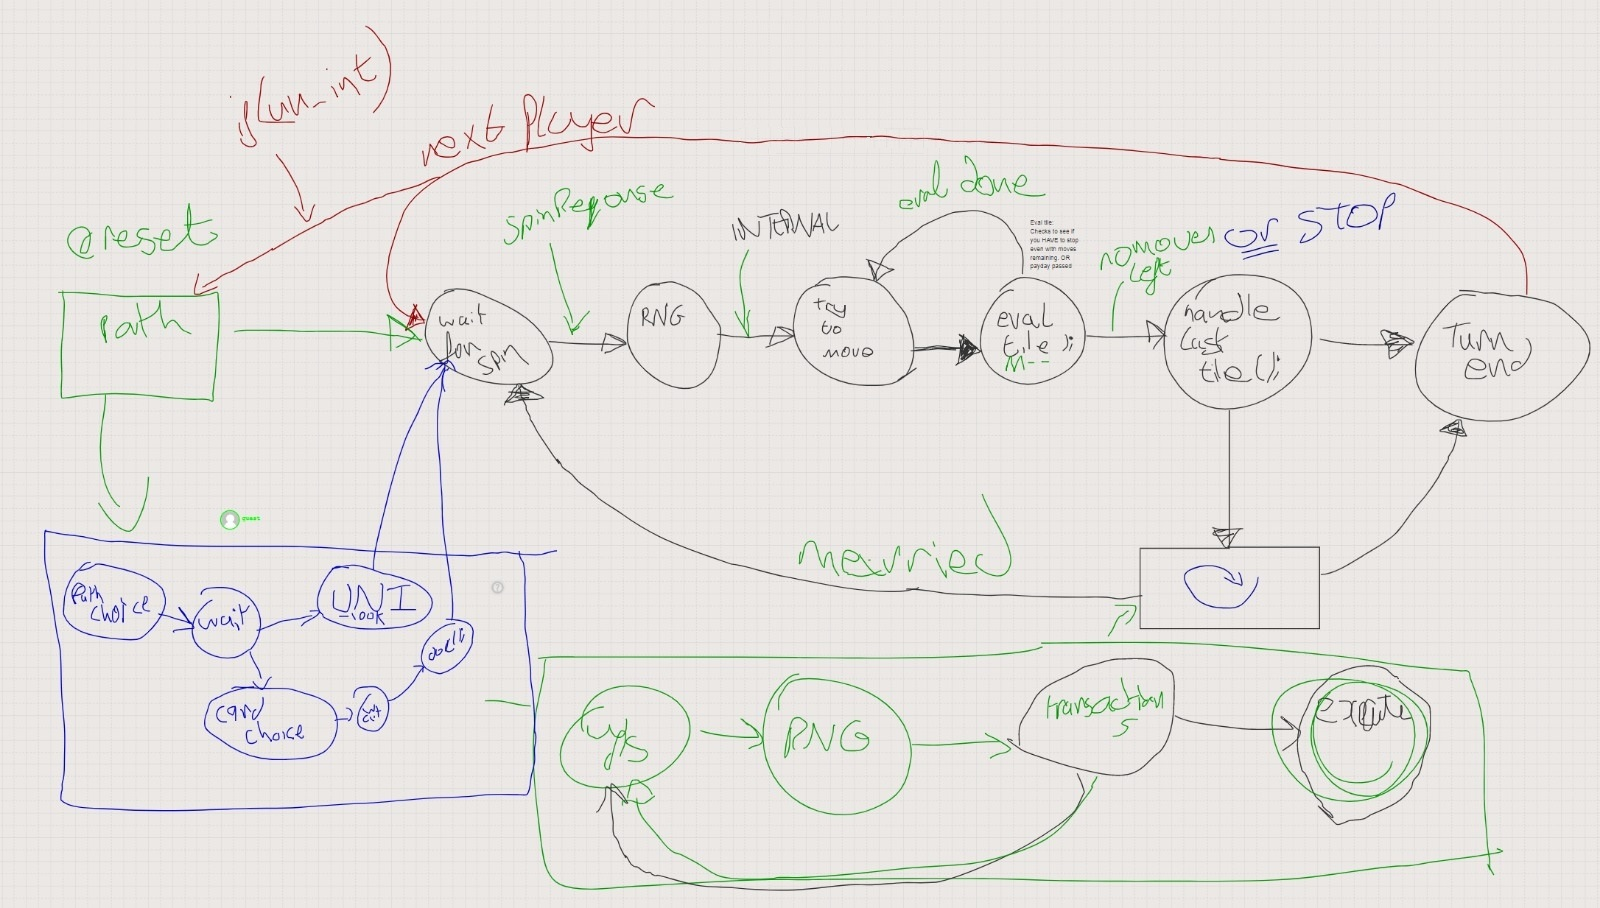
\includegraphics[scale=.4]{highlevel_state_diagram}
		\caption{State Machine Design Doc.}
		\label{fig:state_machine}
	\end{figure}
	\begin{figure}[!h]
		\centering
		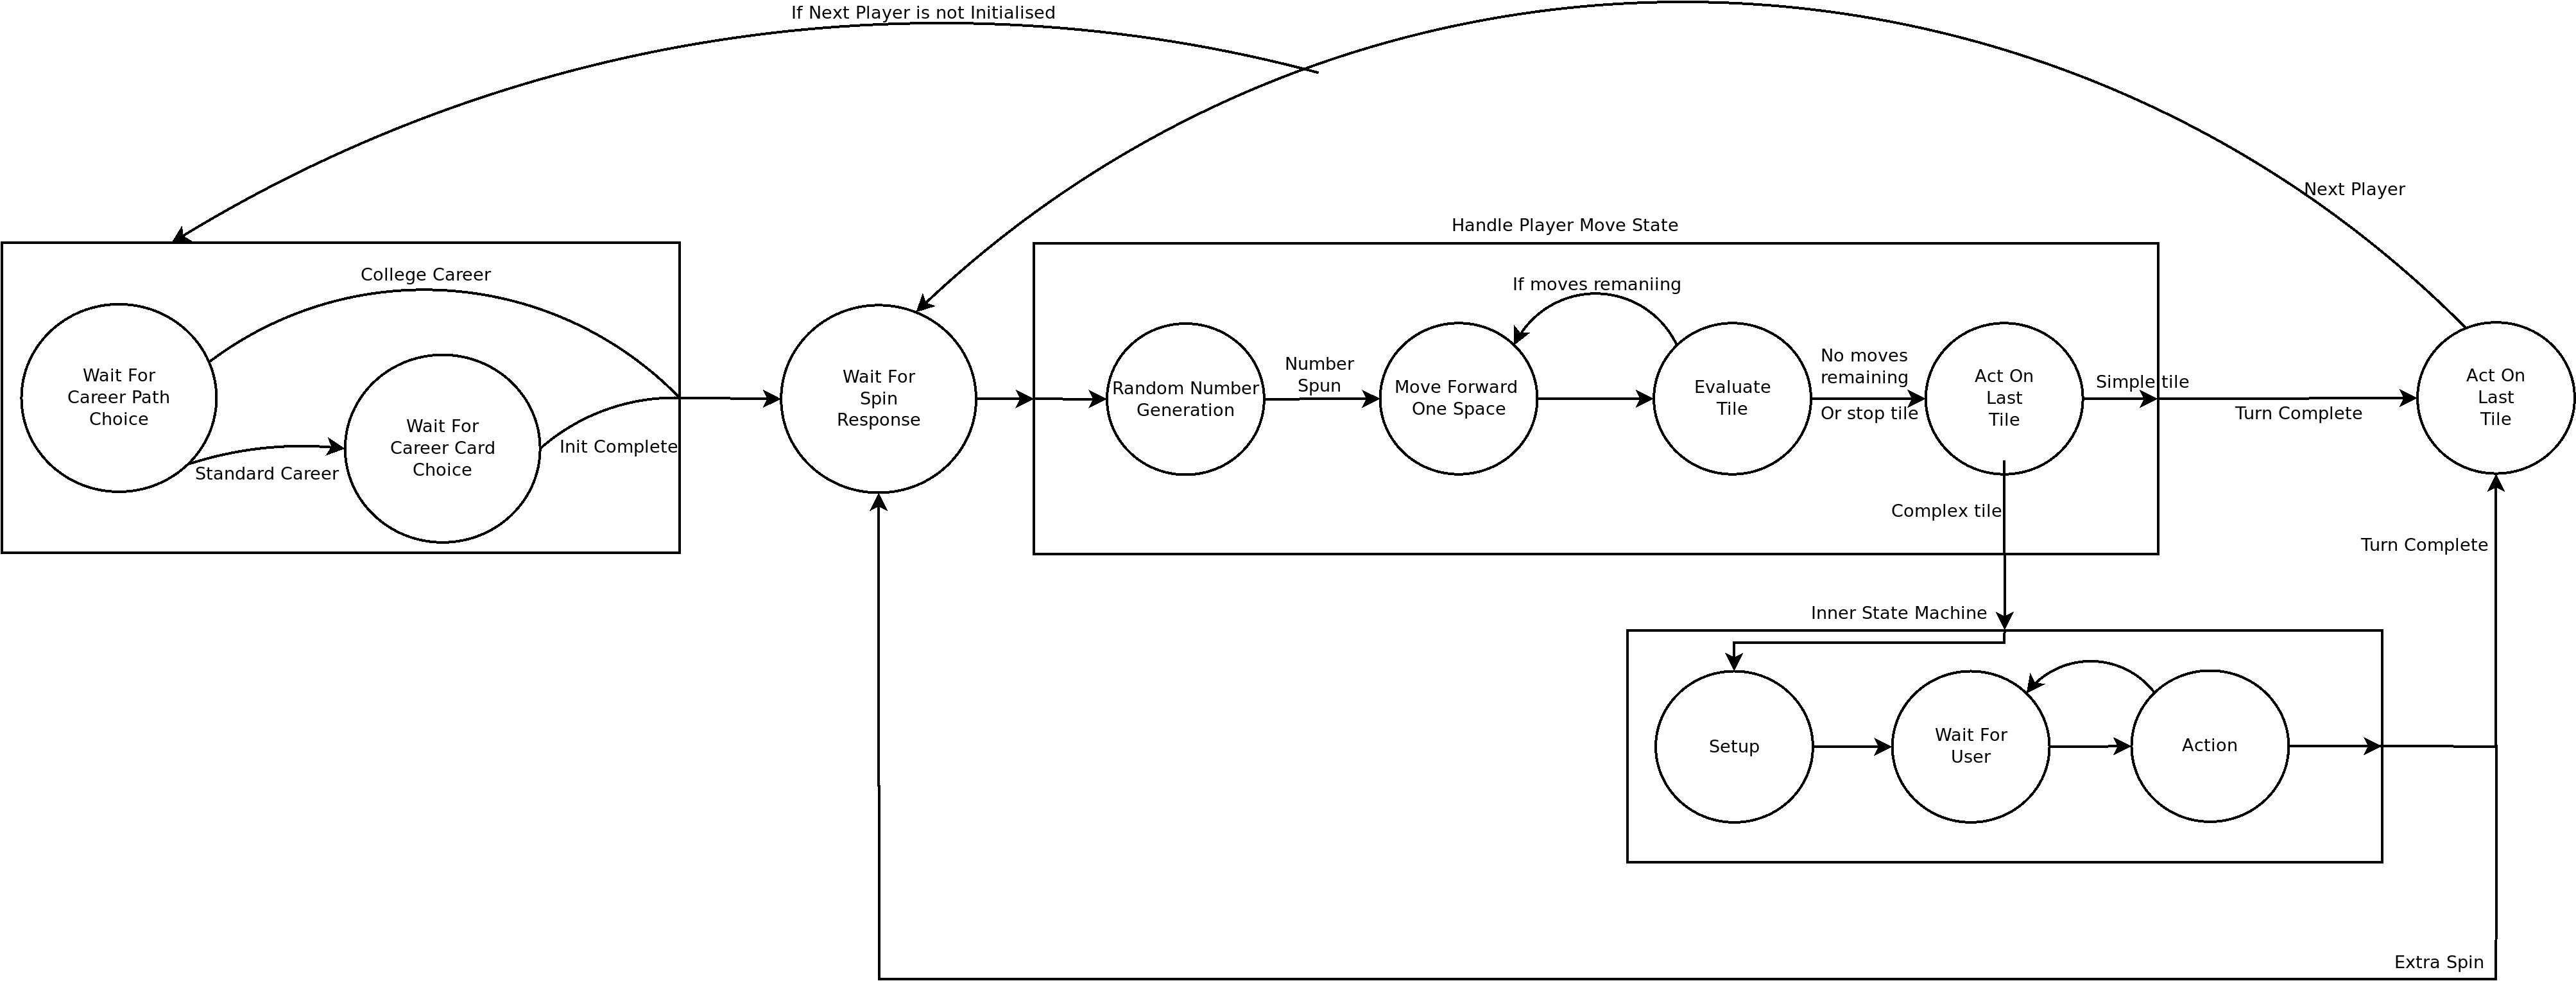
\includegraphics[scale=.1]{state_machine_high_level}
		\caption{State Machine Design as Implemented.}
		\label{fig:state_machine_actual}
	\end{figure}
	\subsection*{UI}
	As previously mentioned the UI runs in two threads. One thread uses backbuffering to draw/render the various UI screens at a fixed frame rate. All interaction is handled by an action listener attached to the various buttons on the display. Depending on which button is activated the UI sends a message to the UI using the messaging system and awaits a response. Depending on this response the UI's state is mutated to represent this information.\\
	For example if the logic sends a message requesting that the user select one career card from two options the selection screen is displayed to the user alongside the relevant buttons and clicking either of these will send a \texttt{DecisionResponse} message as a response to the logic.\\
	Sending a message from the User Interface is a blocking activity in that thread and prevents the user from doing anything until a response has been received from the user.
	\begin{figure}[!h]
		\centering
		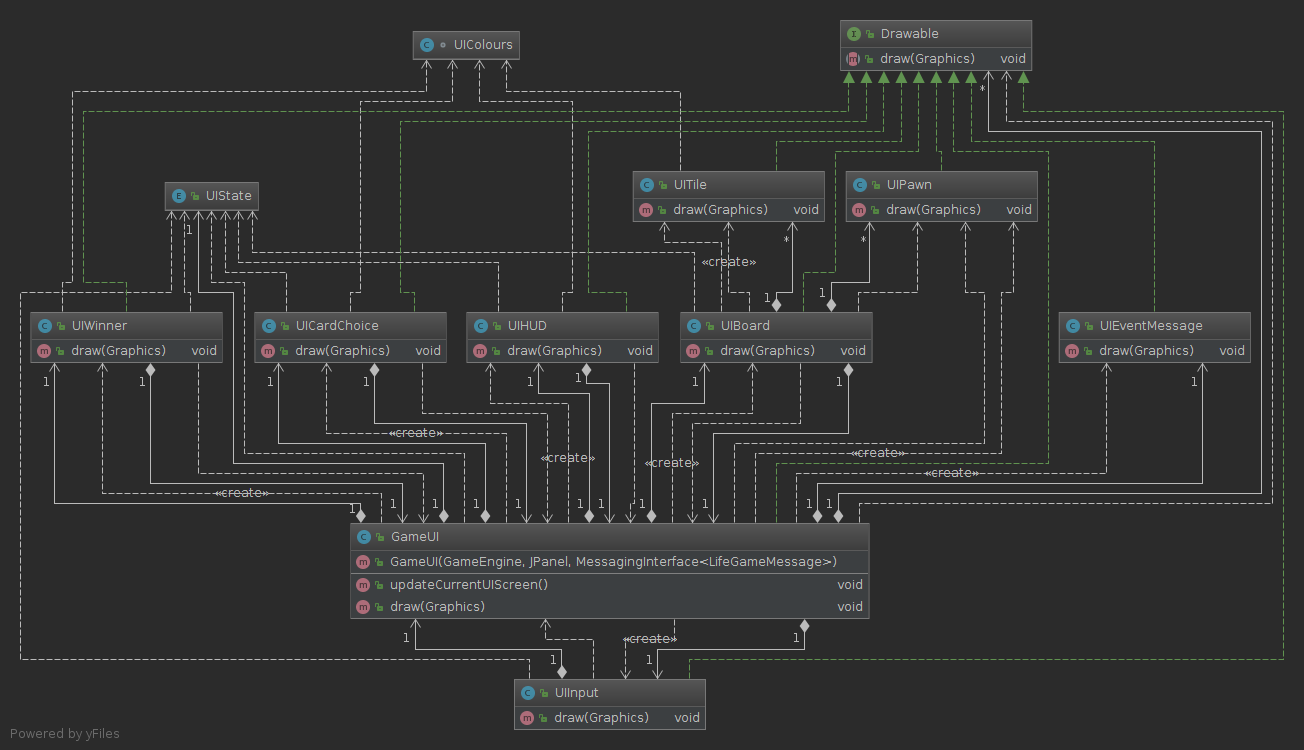
\includegraphics[scale=.35]{uml/ui_uml}
		\caption{UI Internals.}
		\label{fig:ui_uml}
	\end{figure}
	
\end{document}